\begin{name}
	{\tenchude}{\tendethi}{LỚP TOÁN THẦY PHÁT}{\thoigian}
\end{name}
\setcounter{ex}{0}\setcounter{bt}{0}
\Opensolutionfile{ans}[ans/ans-2-TT-13-GiaDinh-HCM-23]

\begin{ex}%[Thi thử, THPT Gia Định HCM 2023]%[Phạm Tuấn, 12-EX6-2023]%[2D2Y5-1]
Nghiệm của phương trình $2023^{x-1}=1$ là
\choice
{$x=2023$}
{\True $x=1$}
{$x=0$}
{$x=4$}
\loigiai{
Ta có $2023^{x-1}=1\Leftrightarrow x-1=0\Leftrightarrow x=1$.
}
\end{ex}

\begin{ex}%[Thi thử, THPT Gia Định HCM 2023]%[Phạm Tuấn, 12-EX6-2023]%[2H2Y1-2]
Cho hình nón có diện tích xung quanh bằng $8\pi $ và độ dài đường sinh là $4$. Tính bán kính đường tròn đáy của hình nón.
\choice
{$2\sqrt{3}$}
{$4$}
{$1$}
{\True $2$}
\loigiai{
Gọi $\ell $, $r$ lần lượt là đường sinh và bán kính đáy của hình nón.\\
Ta có $S_{\text{xq}}=\pi r \ell  \Leftrightarrow 8\pi =\pi \cdot r\cdot 4\Leftrightarrow r=2$.
}
\end{ex}

\begin{ex}%[Thi thử, THPT Gia Định HCM 2023]%[Phạm Tuấn, 12-EX6-2023]%[2D1B2-1]
Số điểm cực trị của hàm số $y=-x^4-4x^3+3$ là
\choice
{$2$}
{$0$}
{$3$}
{\True $1$}
\loigiai{
Ta có $y'=-4x^3-12x^2$; $y'=0\Leftrightarrow -4x^2(x+3)=0\Leftrightarrow \hoac{& x=0 \\& x=-3.}$\\
Bảng xét dấu của $y'$
\begin{center}

\begin{tikzpicture}
	\tkzTabInit[nocadre=false,lgt=1.2,espcl=2.5,deltacl=0.6]
	{$x$ /0.7,$y'$/0.7}
	{$-\infty$,$-3$, $0$, $+\infty$}
	\tkzTabLine{,+,0,-,0,-,}
	\end{tikzpicture}
\end{center}
Suy ra hàm số có đúng $1$ điểm cực trị. 
}
\end{ex}

\begin{ex}%[Thi thử, THPT Gia Định HCM 2023]%[Phạm Tuấn, 12-EX6-2023]%[2D2Y6-1]
Tập nghiệm của bất phương trình $\log _2(x-2)<1$ là
\choice
{$\left(-\infty ;4\right)$}
{$\left(4;+\infty\right)$}
{\True $(2;4)$}
{$\left(2;+\infty\right)$}
\loigiai{
Ta có $\log _2(x-2)<1\Leftrightarrow \heva{& x-2>0 \\& x-2<2 }\Leftrightarrow \heva{& x>2 \\& x<4 }\Leftrightarrow 2<x<4$.\\
Tập nghiệm của bất phương trình $\mathscr{D}=(2;4)$.
}
\end{ex}


\begin{ex}%[Thi thử, THPT Gia Định HCM 2023]%[Phạm Tuấn, 12-EX6-2023]%[1D3Y4-3]
Cấp số nhân $\left(u_n\right)$ có số hạng đầu $u_1=1$, công bội $q=2$, số hạng thứ tư là
\choice
{$u_4=7$}
{$u_4=32$}
{$u_4=16$}
{\True $u_4=8$}
\loigiai{
Ta có $u_4=u_1\cdot q^3=1\cdot 2^3=8$.
}
\end{ex}


\begin{ex}%[Thi thử, THPT Gia Định HCM 2023]%[Phạm Tuấn, 12-EX6-2023]%[2D1Y5-1]
\immini{
Đồ thị hàm số nào dưới đây có dạng của hình bên?
\choice
{\True $y=x^4-2x^2$}
{$y=x^4-2x^2+1$}
{$y=-x^4+2x^2+1$}
{$y=-x^4+2x^2$}
}
{
\begin{tikzpicture}[scale=0.77,>=stealth, font=\footnotesize, line join=round, line cap=round]
%\draw[color=gray!50,dashed] (-3,-2) grid (3,3.5);
\draw[->] (-3,0)--(3,0) node [below]{$x$};
\draw[->] (0,-2)--(0,3.5) node [left]{$y$};
\node at (0,0) [above left]{$O$};
\foreach \x in {-2,-1,1,2} \draw (\x,0.1)--(\x,-0.1) node [below] { $\x$};
\foreach \y in {-1,1,2,3} \draw (0.1,\y)--(-0.1,\y) node [left] { $\y$};
\clip (-3,-3) rectangle (3,3.5);
\draw[smooth,samples=100,domain=-3:3] plot(\x,{(\x)^4-2*(\x)^2});
\end{tikzpicture}
}
\loigiai{
Từ đồ thị hàm số,  ta có  $ \lim \limits_{x\to +\infty } \,y=+\infty $ và đồ thị hàm số  đi qua gốc toạ độ nên  hàm số cần tìm là $y=x^4-2x^2$.
}
\end{ex}

\begin{ex}%[Thi thử, THPT Gia Định HCM 2023]%[Phạm Tuấn, 12-EX6-2023]%[2H3B2-4]
Trong KG $Oxyz$, điểm $M'$ đối xứng với điểm $M\left(2;2;-1\right)$ qua mặt phẳng $(Oyz)$ có tọa độ là
\choice
{$\left(-2;-2;1\right)$}
{\True $\left(-2;2;-1\right)$}
{$\left(-2;0;0\right)$}
{$\left(2;-2;1\right)$}
\loigiai{
Hình chiếu vuông góc của $M\left(2;2;-1\right)$ lên mặt phẳng $(Oyz)$ là điểm $H(0;2;-1)$.\\
$H\left(0;2;-1\right)$ là trung điểm của đoạn thẳng $MM'$ suy ra $ M'\left(-2;2;-1\right)$.
}
\end{ex}


\begin{ex}%[Thi thử, THPT Gia Định HCM 2023]%[Phạm Tuấn, 12-EX6-2023]%[2D3Y3-1]
Cho hàm số $y=f(x)$ xác định và liên tục trên đoạn $\left[a;b\right]$. Diện tích $S$ của hình phẳng được giới hạn bởi đồ thị hàm số $y=f(x)$, trục hoành, đường thẳng $x=a$, $x=b$ được tính theo công thức
\choice
{$S=\displaystyle\int\limits_a^b{f^2(x)}\mathrm{\,d}x$}
{$S=\pi \displaystyle\int\limits_a^b{f^2(x)}\mathrm{\,d}x$}
{$S=\displaystyle\int\limits_a^b{f(x)}\mathrm{\,d}x$}
{\True $S=\displaystyle\int\limits_a^b\left| f(x) \right|\mathrm{\,d}x$}
\loigiai{
Diện tích $S$ của hình phẳng được giới hạn bởi đồ thị hàm số $y=f(x)$, trục hoành, đường thẳng $x=a$, $x=b$ được tính theo công thức $S=\displaystyle\int\limits_a^b\left| f(x) \right|\mathrm{\,d}x$.
}
\end{ex}

\begin{ex}%[Thi thử, THPT Gia Định HCM 2023]%[Phạm Tuấn, 12-EX6-2023]%[2D1Y4-1]
Cho đồ thị hàm số $y=\dfrac{x}{x-2}$. Khẳng định nào sau đây đúng?
\choice
{Đồ thị hàm số không có tiệm cận}
{Đồ thị hàm số có tiệm cận đứng $y=1$}
{Đồ thị hàm số có tiệm cận đứng $x=1$}
{\True Đồ thị hàm số có tiệm cận ngang $y=1$}
\loigiai{
Ta có $ \lim \limits_{x\to 2^+}\dfrac{x}{x-2}=+\infty$ và $ \lim \limits_{x\to - \infty } \dfrac{x}{x-2}=\lim \limits_{x\to + \infty } \dfrac{x}{x-2}= 1$. \\
Suy ra đồ thị hàm số có tiệm cận đứng $x=2$ và tiệm cận ngang $y=1$.
}
\end{ex}


\begin{ex}%[Thi thử, THPT Gia Định HCM 2023]%[Phạm Tuấn, 12-EX6-2023]%[2H3Y2-3]
Trong KG $Oxyz$, phương trình mặt phẳng $(P)$ đi qua điểm $M\left(1;0;1\right)$ và có một  véc-tơ pháp tuyến $\overrightarrow{n}=\left(2;1;-2\right)$ là
\choice
{$-2x+y-2x+4=0$}
{$-2x-y+2z-2=0$}
{$x-z=0$}
{\True $2x+y-2z=0$}
\loigiai{
Phương trình mặt phẳng $(P)$ đi qua điểm $M\left(1;0;1\right)$ và có một  véc-tơ pháp tuyến $\overrightarrow{n} = \left(2;1;-2\right)$ là
$$2(x-1)+(y-0)-2(z-1)=0\Leftrightarrow 2x+y-2z=0.$$
}
\end{ex}


\begin{ex}%[Thi thử, THPT Gia Định HCM 2023]%[Phạm Tuấn, 12-EX6-2023]%[2H3Y1-2]
Trong KG $Oxyz$, véc-tơ $\overrightarrow{a}=(1;2;-2)$ vuông góc với véc-tơ nào sau đây?
\choice
{$\overrightarrow{m}=(2;1;1)$}
{\True $\overrightarrow{p}=(2;1;2)$}
{$\overrightarrow{n}=(-2;-3;2)$}
{$\overrightarrow{q}=(1;-1;2)$}
\loigiai{
Ta có $\overrightarrow{a}\cdot \overrightarrow{p}=1\cdot 2+2\cdot 1+(-2)\cdot 2=0\Rightarrow \overrightarrow{a}\perp \overrightarrow{p}$.
}
\end{ex}


\begin{ex}%[Thi thử, THPT Gia Định HCM 2023]%[Phạm Tuấn, 12-EX6-2023]%[2D4Y1-1]
Số phức liên hợp của số phức $1-3i$ là
\choice
{\True $1+3i$}
{$-1-3i$}
{$3-i$}
{$3+i$}
\loigiai{
Số phức liên hợp của số phức $1-3i$ là $1+3i$.
}
\end{ex}


\begin{ex}%[Thi thử, THPT Gia Định HCM 2023]%[Phạm Tuấn, 12-EX6-2023]%[2D1Y3-1]
Cho hàm số $y=x^3+x+1$. Giá trị lớn nhất của hàm số trên đoạn $[-1;2]$ bằng 
\choice
{$8$}
{$-1$}
{$1$}
{\True $11$}
\loigiai{
Ta có  $y=x^3+x+1$; $y'=3x^2+1>0,\forall x\in \mathbb{R}$.
Suy hàm số đồng biến trên $[-1;2]$. \\
Do đó giá trị lớn nhất của hàm số trên đoạn $[-1;2]$ là $y(2) =  11$.
}
\end{ex}


\begin{ex}%[Thi thử, THPT Gia Định HCM 2023]%[Phạm Tuấn, 12-EX6-2023]%[2D2Y4-1]
Tìm tập xác định của hàm số $y=\ln \left(-x^2+4\right)$.
\choice
{$\mathscr{D}=\left(-\infty ;-1\right]\cup [-2;2]$}
{$\mathscr{D}=\left(-\infty ;-2\right)\cup \left(2;+\infty\right)$}
{$\mathscr{D}=\left(2;+\infty\right)$}
{\True $\mathscr{D}=(-2;2)$}
\loigiai{
Hàm số  xác định khi và chỉ khi $-x^2+4>0\Leftrightarrow -2<x<2$.\\
Suy ra tập xác định của hàm số là $\mathscr{D}=(-2;2)$.
}
\end{ex}


\begin{ex}%[Thi thử, THPT Gia Định HCM 2023]%[Phạm Tuấn, 12-EX6-2023]%[2D3Y1-1]
Trong các hàm số sau đây, hàm số nào là một nguyên hàm của hàm số $f(x)=\dfrac{1}{x-3}$?
\choice
{$y=\dfrac{-1}{(x-3)^2}$}
{$y=\dfrac{1}{(x-3)^2}$}
{\True $y=\ln |x-3|$}
{$y= \dfrac{1}{\ln |x-3|}$}
\loigiai{
Ta có $\displaystyle\int\dfrac{1}{x-3}\mathrm{\,d}x=\ln |x-3|+C$. \\
Vậy hàm số $y=\ln |x-3|$ là một nguyên hàm của hàm số $f(x)=\dfrac{1}{x-3}$.
}
\end{ex}

\begin{ex}%[Thi thử, THPT Gia Định HCM 2023]%[Phạm Tuấn, 12-EX6-2023]%[2H2Y1-1]
Cho khối trụ $(T)$ có bán kính đáy bằng $2$ và chiều cao bằng $4$. Thể tích khối trụ $(T)$ bằng
\choice
{$32\pi $}
{$8\pi $}
{$24\pi $}
{\True $16\pi $}
\loigiai{
Thể tích khối trụ $(T)$ là $V=\pi \cdot r^2\cdot h=\pi \cdot 2^2\cdot 4=16\pi$.
}
\end{ex}


\begin{ex}%[Thi thử, THPT Gia Định HCM 2023]%[Phạm Tuấn, 12-EX6-2023]%[2H1B3-2]
Thể tích của khối lăng trụ tam giác đều tất cả các cạnh bằng $2$ là
\choice
{$2\sqrt{2}$}
{$\dfrac{2\sqrt{3}}{3}$}
{$\dfrac{2\sqrt{2}}{3}$}
{\True $2\sqrt{3}$}
\loigiai{
Khối lăng trụ tam giác đều có tất cả các cạnh bằng $2$ nên có chiều cao $h=2$ và diện tích đáy là $S=\dfrac{\sqrt{3}}{4}{{\cdot 2}^2}=\sqrt{3}$.\\
Vậy thể tích khối lăng trụ là $V=S\cdot h=2\sqrt{3}$.
}
\end{ex}


\begin{ex}%[Thi thử, THPT Gia Định HCM 2023]%[Phạm Tuấn, 12-EX6-2023]%[2D1Y1-2]
Cho hàm số $y=f(x)$ có bảng biến thiên như sau
\begin{center}

\begin{tikzpicture}[>=stealth]
\tkzTabInit[nocadre=false,lgt=1.2,espcl=2.5,deltacl=0.6]
{$x$ /0.6,$y'$ /0.6,$y$ /2}
{$-\infty$,$0$,$2$,$+\infty$}
\tkzTabLine{,-,$0$,+,$0$,-,}
\tkzTabVar{+/$+\infty$, -/$-4$,+/$1$,-/$-\infty$}
\end{tikzpicture}
\end{center}
Hàm số đã cho đồng biến trên khoảng nào dưới đây?
\choice
{$(-4;1)$}
{$\left(2;+\infty\right)$}
{\True $\left(0;2\right)$}
{$\left(-\infty;0\right)$}
\loigiai{
Hàm số đã cho đồng biến trên khoảng $\left(0;2\right)$.
}
\end{ex}


\begin{ex}%[Thi thử, THPT Gia Định HCM 2023]%[Phạm Tuấn, 12-EX6-2023]%[2D1B1-3]
Số giá trị nguyên của tham số $m$ để hàm số $y=x^3-3mx^2+3x+1$ đồng biến trên $\mathbb{R}$ là
\choice
{\True $3$}
{$1$}
{Vô số}
{$5$}
\loigiai{
Ta có $y'=3x^2-6mx+3$.\\
Hàm số đồng biến trên $\mathbb{R}$ khi và chỉ khi $y' \geq 0$, $\forall x \in \mathbb{R}$ 
$$\Leftrightarrow \Delta' \leq 0\Leftrightarrow 9m^2-9\leq 0\Leftrightarrow -1\leq m\leq 1.$$
Theo giả thiết $m\in \mathbb{Z}$ nên $m\in \left\{ -1;0;1 \right\}$.\\
Vậy có $3$ giá trị nguyên $m$ cần tìm.
}
\end{ex}


\begin{ex}%[Thi thử, THPT Gia Định HCM 2023]%[Phạm Tuấn, 12-EX6-2023]%[2H1B3-3]
Cho hình chóp $S.ABC$ có $A'$, $B'$ lần lượt là trung điểm của $SA$, $SB$. Mặt phẳng $\left(CA'B'\right)$ chia khối chóp thành hai khối đa diện có thể tích lần lượt là $V_1$, $V_2$ $\left(V_1>V_2\right)$. Tỉ số $\dfrac{V_1}{V_2}$ gần với số nào nhất dưới đây?
\choice
{$3{,}9$}
{\True $2{,}9$}
{$2{,}5$}
{$0{,}33$}
\loigiai{
\immini{
Mặt phẳng $\left(CA'B'\right)$ chia khối chóp $S.ABC$ thành khối chóp $S.A'B'C$ và khối đa diện $ABCA'B'$. \\
Ta có $\dfrac{V_{S.A'B'C}}{V_{S.ABC}} = \dfrac{SA'}{SA} \cdot \dfrac{SB'}{SB} = \dfrac{1}{4}$. \\
Suy ra $V_2= V_{S.A'B'C} =\dfrac{1}{4} V_{S.ABC}$ và $V_1= V_{ABCA'B'} =\dfrac{3}{4} V_{S.ABC}$. \\
Vậy $\dfrac{V_1}{V_2}=3$.
}{
\begin{tikzpicture}[scale=0.77,>=stealth, font=\footnotesize, line join=round, line cap=round]
\path 	(0,0) coordinate (A)
($(A)+(0:4)$) coordinate (C)
($(A)+(-50:2)$) coordinate (B)
($(B)+(88:4.8)$) coordinate (S)
($(S)!0.5!(B)$) coordinate (B')
($(S)!0.5!(A)$) coordinate (A');
\draw[dashed] 	(A)--(C) (A')--(C) ;
\draw		(B)--(A)--(S)--(C)--(B)--(S) (A')--(B')--(C) ;
\foreach \x/\g in {A/180,B/-90,C/0,S/90,A'/180,B'/-135}
\fill[black] 	(\x) circle (1pt) ($(\g:3mm)+(\x)$) node {$\x$};
\end{tikzpicture}
}
}
\end{ex}

\begin{ex}%[Thi thử, THPT Gia Định HCM 2023]%[Phạm Tuấn, 12-EX6-2023]%[2D1B5-6]
Cho $M$ là giao điểm của đồ thị hàm số $y=\dfrac{x+1}{x-2}$ với trục hoành. Phương trình tiếp tuyến với đồ thị hàm số trên tại điểm $M$ là
\choice
{$3y-x-1=0$}
{$3y+x-1=0$}
{$3y-x+1=0$}
{\True $3y+x+1=0$}
\loigiai{
Ta có $y' = -\dfrac{3}{(x-2)^2}$. \\
$\dfrac{x+1}{x-2}=0 \Leftrightarrow    x=-1$.  
Suy ra giao điểm của đồ thị hàm số $y=\dfrac{x+1}{x-2}$ với trục hoành là $M(-1;0)$.\\
Phương trình tiếp tuyến của đồ thị hàm số đã cho tại điểm $M$ là
\[
y=y'\left(-1\right)\left(x+1\right)+y(-1)=-\dfrac{1}{3}(x+1)\Leftrightarrow 3y+x+1=0.
\]
}
\end{ex}


\begin{ex}%[Thi thử, THPT Gia Định HCM 2023]%[Phạm Tuấn, 12-EX6-2023]%[2D2Y3-2]
Với $a$, $b$ là các số thực dương bất kì, $\log _2\left(ab^3\right)$ bằng
\choice
{$\log _2a+\log _23b$}
{$3\log _2(ab)$}
{$\log _2a-3\log _2b$}
{\True $\log _2a+3\log _2b$}
\loigiai{
Ta có $\log _2\left(ab^3\right)=\log _2a+\log _2b^3=\log _2a+3\log _2b$.
}
\end{ex}


\begin{ex}%[Thi thử, THPT Gia Định HCM 2023]%[Phạm Tuấn, 12-EX6-2023]%[1D2B5-2]
Một túi đựng $5$ bi xanh và $5$ bi đỏ. Lấy ngẫu nhiên $2$ bi, xác suất để cả hai bi đều màu đỏ là
\choice
{$\dfrac{1}{3}$}
{\True $\dfrac{2}{9}$}
{$\dfrac{2}{5}$}
{$\dfrac{8}{9}$}
\loigiai{
Ta có $n(\Omega) = \mathrm{C}_{10}^2$. \\
Gọi $A$ là biến cố ``Cả hai bi đều màu đỏ''.
Ta có $n(A)= \mathrm{C}_5^2$. \\
Vậy   $\mathrm{P}(A)=\dfrac{n(A)}{n(\Omega)} =  \dfrac{\mathrm{C}_5^2}{\mathrm{C}_{10}^2}=\dfrac{2}{9}$.
}
\end{ex}


\begin{ex}%[Thi thử, THPT Gia Định HCM 2023]%[Phạm Tuấn, 12-EX6-2023]%[2D2B5-2]
Tổng hai nghiệm của phương trình $2^{x^2+x+1}=8^{2x}$ bằng
\choice
{\True $5$}
{$6$}
{$1$}
{$8$}
\loigiai{
Ta có ${2^{x^2+x+1}}={8^{2x}}={2^{6x}}\Leftrightarrow x^2-5x+1=0 \Leftrightarrow x= \dfrac{5\pm \sqrt{21}}{2}$. \\
Vậy  tổng các nghiệm của phương trình bằng $5$.
}
\end{ex}


\begin{ex}%[Thi thử, THPT Gia Định HCM 2023]%[Phạm Tuấn, 12-EX6-2023]%[2D2B6-3]
Số nghiệm nguyên của bất phương trình $\log_{\tfrac{1}{4}}(x-1)+\log _4(14-2x)\ge 0$ là
\choice
{$6$}
{$3$}
{\True $4$}
{$5$}
\loigiai{
Điều kiện xác định:  $\heva{& x-1>0 \\& 14-2x>0 }\Leftrightarrow 1<x<7$.\\
Bất phương trình tương đương
\begin{align*}
& \log_{\tfrac{1}{4}}(x-1)+\log_4(14-2x) \geq 0 \\ 
\Leftrightarrow ~& \log_4(14-2x) \geq  \log_{4}(x-1) \\
\Leftrightarrow ~& 14-2x\ge x-1 \\
 \Leftrightarrow~ & x \leq 5.
\end{align*}
Suy ra  tập nghiệm của bất phương trình trên là $S=(1;5]$.\\
Vậy số nghiệm nguyên của bất phương trình bằng $4$.
}
\end{ex}

\begin{ex}%[Thi thử, THPT Gia Định HCM 2023]%[Phạm Tuấn, 12-EX6-2023]%[2H3B3-2]
Trong KG $Oxyz$, đường thẳng $d$ đi qua điểm $M(1;2;-1)$, đồng thời vuông góc với mặt phẳng $(P)\colon x+y-z+1=0$ có phương trình là
\choice
{$\dfrac{x+1}{-1}=\dfrac{y+2}{-2}=\dfrac{z+1}{1}$}
{$\dfrac{x-1}{1}=\dfrac{y-1}{2}=\dfrac{z+1}{-1}$}
{$\dfrac{x-1}{1}=\dfrac{y+2}{1}=\dfrac{z+1}{-1}$}
{\True $\dfrac{x-1}{1}=\dfrac{y-2}{1}=\dfrac{z+1}{-1}$}
\loigiai{
Do $d\perp (P)$ nên $\overrightarrow{u}_d=\overrightarrow{n}_P=(1;1;-1)$ là một véc-tơ chỉ phương của đường thẳng $d$.\\
Đường thẳng $d$ đi qua điểm $M(1;2;-1)$ và có một véc-tơ chỉ phương $\overrightarrow{u}_d=(1;1;-1)$ có phương trình là $$\dfrac{x-1}{1}=\dfrac{y-2}{1}=\dfrac{z+1}{-1}.$$
}
\end{ex}


\begin{ex}%[Thi thử, THPT Gia Định HCM 2023]%[Phạm Tuấn, 12-EX6-2023]%[2D4B2-2]
Cho số phức $z=1+i$. Môđun của số phức $w=(1+3i)z$ là
\choice
{$ 20 $}
{$\sqrt{2}$}
{$\sqrt{10}$}
{\True $\sqrt{20}$}
\loigiai{
Ta có $w=(1+3i)z=(1+3i)(1+i)=-2+4i$.\\
Vậy $|w|=\sqrt{(-2)^2+4^2}=\sqrt{20}$.
}
\end{ex}


\begin{ex}%[Thi thử, THPT Gia Định HCM 2023]%[Phạm Tuấn, 12-EX6-2023]%[2D3B2-2]
Cho hàm số $f(x)$ có đạo hàm liên tục trên đoạn $[2;4]$ và thỏa mãn $f(2)=3$, $f(4)=2023$. Tính tích phân $I=\displaystyle\int\limits_1^2{f'(2x)\mathrm{\,d}x}$.
\choice
{$I=1011$}
{$I=2022$}
{$I=2020$}
{\True $I=1010$}
\loigiai{
Ta có 
\begin{align*}
I&=\displaystyle\int\limits_1^2{f'(2x)\mathrm{\,d}x}=\dfrac{1}{2}\displaystyle\int\limits_1^2{f'(2x)\text{\,d}(2x)} \\
&=\dfrac{1}{2}f(2x) \bigg|_1^2=\dfrac{1}{2}\left(f(4)-f(2)\right)=\dfrac{1}{2}(2023-3)=1010. 
\end{align*}
}
\end{ex}


\begin{ex}%[Thi thử, THPT Gia Định HCM 2023]%[Phạm Tuấn, 12-EX6-2023]%[2H3B3-4]
Trong KG $Oxyz$, cho đường thẳng $\triangle \colon \dfrac{x-2}{1}=\dfrac{y+2}{2}=\dfrac{z}{-2}$ và mặt phẳng $(P)\colon 2x-y+2z-2022=0$. Gọi $\alpha $ là góc giữa đường thẳng $\Delta $ và mặt phẳng $(P)$. Khẳng định nào sau đây đúng?
\choice
{$\sin \alpha =-\dfrac{4}{9}$}
{\True $\sin \alpha =\dfrac{4}{9}$}
{$\cos \alpha =-\dfrac{4}{9}$}
{$\cos \alpha =\dfrac{4}{9}$}
\loigiai{
Đường thẳng $\Delta$ có một véc-tơ chỉ phương $\overrightarrow{u}=(1;2;-2)$; mặt phẳng $(P)$ có một  véc-tơ pháp tuyến $\overrightarrow{n}=(2;-1;2)$.\\
Ta có $\sin \alpha =\left| \cos \left(\overrightarrow{n},\overrightarrow{u}\right) \right|=\dfrac{\left| \overrightarrow{n}\cdot \overrightarrow{u} \right|}{\left| {\overrightarrow{n}} \right|\cdot \left| {\overrightarrow{u}} \right|}=\dfrac{|1\cdot 2 + 2 \cdot (-1) +(-2) \cdot 2|}{\sqrt{1^2+2^2+(-2)^2} \cdot \sqrt{2^2+(-1)^2+2^2}} =\dfrac{4}{9}$.
}
\end{ex}


\begin{ex}%[Thi thử, THPT Gia Định HCM 2023]%[Phạm Tuấn, 12-EX6-2023]%[2D3B3-3]
Cho hình phẳng $(H)$ giới hạn bởi đồ thị $(P)\colon y=2x-x^2$ và trục $Ox$. Tính thể tích của khối tròn xoay tạo thành khi cho $(H)$ quay quanh trục $Ox$.
\choice
{$V=\dfrac{19\pi }{15}$}
{$V=\dfrac{13\pi }{15}$}
{$V=\dfrac{17\pi }{15}$}
{\True $V=\dfrac{16\pi }{15}$}
\loigiai{
Phương trình hoành độ giao điểm của đồ thị $(P)$ và trục $Ox$ là $2x-x^2=0\Leftrightarrow \hoac{& x=0 \\& x=2.}$\\
Thể tích khối tròn xoay cần tìm là $V=\pi \displaystyle\int\limits_0^2{{{\left(2x-x^2\right)}^2}\mathrm{\,d}x}=\dfrac{16\pi }{5}$.
}
\end{ex}

\begin{ex}%[Thi thử, THPT Gia Định HCM 2023]%[Phạm Tuấn, 12-EX6-2023]%[2H2B2-3]
Thể tích khối cầu nội tiếp hình lập phương cạnh $2a$ là
\choice
{$V=\dfrac{\sqrt{3}\pi a^3}{2}$}
{$V=4\sqrt{3}\pi a^3$}
{\True $V=\dfrac{4\pi a^3}{3}$}
{$V=\dfrac{32\pi a^3}{3}$}
\loigiai{
Khối cầu nội tiếp hình lập phương cạnh $2a$ có bán kính là $R=\dfrac{2a}{2}=a$.\\
Thể tích khối cầu là $V=\dfrac{4}{3}\pi R^3 =  \dfrac{4\pi a^3}{3}$.
}
\end{ex}


\begin{ex}%[Thi thử, THPT Gia Định HCM 2023]%[Phạm Tuấn, 12-EX6-2023]%[2H1B3-2]
Cho hình chóp $S.ABC$ có đáy $ABC$ là tam giác đều cạnh $a,SA\perp (ABC)$ và góc giữa đường thẳng $SB$ và mặt phẳng $(ABC)$ bằng $60^\circ$. Thể tích khối chóp $S.ABC$ bằng
\choice
{$\dfrac{a^3}{2}$}
{$\dfrac{3a^3}{8}$}
{$\dfrac{3a^3}{4}$}
{\True $\dfrac{a^3}{4}$}
\loigiai{
\immini{
The giả thiết $SA \perp (ABC)$ nên $\left(SB,(ABC)\right)=\left(SB,AB\right)=\widehat{SBA}=60^\circ$.\\
$\triangle SAB$ vuông tại $A$ nên $SA=AB\tan \widehat{SBA}=a\tan 60^\circ=a\sqrt{3}$.\\
Thể tích khối chóp $S.ABC$ là $$V=\dfrac{1}{3}\cdot SA\cdot S_{\triangle ABC}=\dfrac{1}{3}\cdot a\sqrt{3}\cdot \dfrac{a^2\sqrt{3}}{4}=\dfrac{a^3}{4}$$
}
{
\begin{tikzpicture}[scale=0.7, font=\footnotesize, line join=round, line cap=round, >=stealth]
\path
(0,0) coordinate (A)
(1,-1) coordinate (B)
(4,0) coordinate (C)
(0,3.5) coordinate (S) ;
\draw (A)--(B)--(C)--(S)--cycle (S)--(B);
\draw[dashed] (A)--(C);
\foreach \x/\g in{A/180,B/-90,C/0,S/90}
\fill[black](\x)circle(1.4pt) ($(\x)+(\g:3.5mm)$) node{$\x$}; 
\end{tikzpicture}
}
}
\end{ex}


\begin{ex}%[Thi thử, THPT Gia Định HCM 2023]%[Phạm Tuấn, 12-EX6-2023]%[1H3B4-3]
Cho hình lăng trụ tam giác đều $ABC. A'B'C'$ có cạnh đáy bằng $a$, cạnh bên bằng $\dfrac{3a}{2}$. Góc giữa hai mặt phẳng $\left(A'BC\right)$ và mặt phẳng $(ABC)$ bằng
\choice
{$45^\circ $}
{$90^\circ $}
{\True $60^\circ $}
{$30^\circ $}
\loigiai{
\immini{
Gọi $M$ là trung điểm $BC$. \\
Ta có $\heva{&BC \perp AM\\&BC\perp AA'}$ suy ra $BC\perp (AA'M)$, do đó $\left(\left(A'BC\right),(ABC)\right)=\widehat{A'MA}$.\\
Ta có $AM=\dfrac{a\sqrt{3}}{2}$, $\tan \widehat{A'MA}=\dfrac{AA'}{AM}=\sqrt{3}\Rightarrow \widehat{A'MA}={{60}^{\circ }}$. \\
Vậy góc giữa hai mặt phẳng $\left(A'BC\right)$ và mặt phẳng $(ABC)$ bằng $60^\circ $.
}
{
\begin{tikzpicture}[scale=0.77, font=\footnotesize, line join=round, line cap=round, >=stealth]
\path
(0,0) coordinate (A)
(1.25,-1.5) coordinate (B)
(3,0) coordinate (C)
(0,3) coordinate (A')
($(A')+(B)-(A)$) coordinate (B')
($(A')+(C)-(A)$) coordinate (C')
($(C)!.5!(B)$) coordinate (M)
;
\draw (A)--(B)--(C)--(C')--(B')--(A')--(C') (A)--(A') (B)--(B') (A')--(B);
\draw[dashed] (A)--(C) (A)--(M)--(A')--(C);
\foreach \x/\g in{A/180,B/-90,C/0,A'/120,B'/-20,C'/30,M/-30}
\fill[black](\x)circle(1.1pt) ($(\x)+(\g:3mm)$) node{$\x$}; 
\end{tikzpicture}
}
}
\end{ex}


\begin{ex}%[Thi thử, THPT Gia Định HCM 2023]%[Phạm Tuấn, 12-EX6-2023]%[2D2B4-3]
\immini{
Cho hàm số $y=\log _ax$ $\left(0<a\ne 1\right)$ có đồ thị như hình bên. Giá trị của $a$ bằng
\choice
{\True $\sqrt{2}$}
{$\dfrac{1}{\sqrt{2}}$}
{$\dfrac{1}{2}$}
{$2$}
}
{
\begin{tikzpicture}[>=stealth,scale=0.7, line join=round, line cap=round,font=\footnotesize]
\draw[->] (-2,0)--(4,0) node [below]{$x$};
\draw[->] (0,-2)--(0,4) node [left]{$y$};
\node at (0,0) [below left]{$O$};
\fill[black] (1,0) circle (1pt) node [below] {$1$}
(0,2) circle (1pt) node[left] {$2$} (2,0) circle (1pt) node [below] {$2$}  (2,2) circle (1pt);
\clip (-5,-2) rectangle (5.5,4.5);
\draw[smooth,samples=150,domain=0.1:4] plot(\x,{ln(\x)/ln(sqrt(2))});
\draw[dashed] (0,2)--(2,2)--(2,0);
\node at (1,3.5)[right]{$y=\log_ax$};
\end{tikzpicture}
}
\loigiai{
Đồ thị hàm số đi qua điểm $(2;2)$ nên $2=\log _a2\Leftrightarrow a=\sqrt{2}$.
}
\end{ex}


\begin{ex}%[Thi thử, THPT Gia Định HCM 2023]%[Phạm Tuấn, 12-EX6-2023]%[2H2B1-2]
Trong không gian, cho hình chữ nhật $ABCD$ có $AB=2$, $AD=1$. Quay hình chữ nhật đó xung quanh cạnh $AB$, ta được một hình trụ. Diên tích xung quanh của hình trụ là
\choice
{$2\pi $}
{$\dfrac{2\pi }{3}$}
{$\dfrac{4\pi }{3}$}
{\True $4\pi $}
\loigiai{
Quay hình chữ nhật quanh cạnh $AB$ ta được một khối trụ có chiều cao $h=AB$ và bán kính đáy là $r=AD$.\\
Khi đó diện tích xung quanh của hình trụ là $S=2\pi rh=2\cdot \pi \cdot 1 \cdot 2=4\pi $
}
\end{ex}

\begin{ex}%[Thi thử, THPT Gia Định HCM 2023]%[Phạm Tuấn, 12-EX6-2023]%[2D2G6-4]
Có bao nhiêu số nguyên $x$ thỏa mãn $\log_3\dfrac{x^2-9}{125}\le \log_5\dfrac{x^2-9}{27}$?
\choice
{$116$}
{$58$}
{$117$}
{\True $110$}
\loigiai{
Điều kiện xác định: $\hoac{&x>3\\&x<-3.}$ \\
 Ta có
\begin{eqnarray*}
&&\log_3\dfrac{x^2-9}{125}\le \log_5\dfrac{x^2-9}{27}\\
&\Leftrightarrow&\dfrac{1}{\ln 3}\left(\ln \left(x^2-9\right)-\ln 125\right)\le \dfrac{1}{\ln 5}\left(\ln \left(x^2-9\right)-\ln 27\right) \\
& \Leftrightarrow& \dfrac{1}{\ln 3}\left(\ln \left(x^2-9\right)-3\ln 5\right)\le \dfrac{1}{\ln 5}\left(\ln \left(x^2-9\right)-3\ln 3\right)\\
& \Leftrightarrow& \left(\ln 5-\ln 3\right)\ln \left(x^2-9\right)\le 3\left(\ln ^25-{{\ln }^2}3\right)\\
&\Leftrightarrow& \ln \left(x^2-9\right)\le 3\left(\ln 5+\ln 3\right)\\
&\Leftrightarrow& x^2-9\le {{15}^3} \\
&\Leftrightarrow& -\sqrt{3384}\le x\le \sqrt{3384}.
\end{eqnarray*}
Kết hợp điều kiện suy ra bất phương trình có tập nghiệm là $S=[-\sqrt{3384};-3) \cup (3; \sqrt{3384}]$. \\
Mặt khác, $x$ nguyên suy ra  $x\in \left\{ -58;-57;\ldots;-4;4;\ldots ;57;58 \right\}$.\\
Vậy có $ 110 $ số nguyên $ x $ thỏa mãn
}
\end{ex}


\begin{ex}%[Thi thử, THPT Gia Định HCM 2023]%[Phạm Tuấn, 12-EX6-2023]%[2H3B3-2]
Trong KG $Oxyz$, cho điểm $M(-1;1;3)$ và hai đường thẳng $\Delta \colon \dfrac{x-1}{3}=\dfrac{y+3}{2}=\dfrac{z-1}{1}$, \\
$\Delta' \colon \dfrac{x+1}{1}=\dfrac{y}{3}=\dfrac{z}{-2}$. Phương trình nào dưới đây là PTĐT đi qua $M$ và vuông góc với $\Delta$ và $\Delta'$?
\choice
{$\heva{& x=-1-t \\& y=1+t \\& z=1+3t }$}
{$\heva{& x=-t \\& y=1+t \\& z=3+t }$}
{$\heva{& x=-1-t \\& y=1-t \\& z=3+t }$}
{\True $\heva{& x=-1-t \\& y=1+t \\& z=3+t }$}
\loigiai{
Véc-tơ  chỉ phương  của $\Delta$, $\Delta'$ lần lượt là $\overrightarrow{u}=(3;2;1)$ và $\overrightarrow{v}=(1;3;-2)$, do đó $\left[\overrightarrow{u},\overrightarrow{v}\right]=(-7;7;7)$.\\
Theo giả thiết $d$ vuông góc với $\Delta$ và $\Delta'$ nên $d$ có một véc-tơ chỉ phương $\overrightarrow{u}_d=(-1;1;1)$. \\
Vậy đường thẳng $d$ có phương trình là  $\heva{& x=-1-t \\& y=1+t \\& z=3+t.}$
}
\end{ex}


\begin{ex}%[Thi thử, THPT Gia Định HCM 2023]%[Phạm Tuấn, 12-EX6-2023]%[2H1B3-2]
Cho lăng trụ đều $ABC.A'B'C'$ có cạnh đáy bằng $a$, góc giữa đường thẳng $AB'$ và mặt phẳng $(BCC'B')$ bằng $30^\circ$. Tính thể tích khối lăng trụ $ABC. A'B'C'$.
\choice
{$\dfrac{a^3}{4}$}
{$\dfrac{\sqrt{6}a^3}{12}$}
{\True $\dfrac{\sqrt{6}a^3}{4}$}
{$\dfrac{a^3}{4}$}
\loigiai{
\immini{
Gọi $M$ là trung điểm $BC$.\\
Ta có $\heva{& AM\perp BC \\& AM\perp BB' }\Rightarrow AM\perp (BCC'B')$. \\
Do đó góc giữa đường thẳng $AB'$ và mặt phẳng $(BCC'B')$ bằng góc $\widehat{AB'M}$.\\
Tam giác $\triangle AB'M$ có $\widehat{AB'M}=30^\circ$, $\widehat{AMB'}=90^\circ$, $AM=\dfrac{a\sqrt{3}}{2}$ 
nên $AB'=\dfrac{AM}{\sin 30^\circ}=a\sqrt{3}$.\\
Suy ra $AA'=\sqrt{A{{{B'}}^2}-A'{{{B'}}^2}}=\sqrt{3a^2-a^2}=a\sqrt{2}$.\\
Vậy $V_{ABC. A'B'C'}=AA'\cdot {S}_{\triangle ABC}=a\sqrt{2}\cdot \dfrac{a^2\sqrt{3}}{4}=\dfrac{a^3\sqrt{6}}{4}$.
}
{
\begin{tikzpicture}[scale=0.77, font=\footnotesize, line join=round, line cap=round, >=stealth]
\path
(0,0) coordinate (A)
(1.25,-1.4) coordinate (B)
(3,0) coordinate (C)
(0,3) coordinate (A')
($(A')+(B)-(A)$) coordinate (B')
($(A')+(C)-(A)$) coordinate (C')
($(C)!.5!(B)$) coordinate (M)
;

\draw (A)--(B)--(C)--(C')--(A')--(B')--(C') (A)--(A') (B)--(B') (A)--(B')--(M);
\draw[dashed] (A)--(C) (C')--(A)--(M);
\foreach \x/\g in{A/180,B/-90,C/0,A'/120,B'/190,C'/30,M/-30}
\fill[black](\x)circle(1.1pt) ($(\x)+(\g:3mm)$) node{$\x$}; 
\end{tikzpicture}
}
}
\end{ex}


\begin{ex}%[Thi thử, THPT Gia Định HCM 2023]%[Phạm Tuấn, 12-EX6-2023]%[2D3K1-1]
Cho hàm số $y=f(x)$ xác định $\mathbb{R} \setminus \{0\}$ thoả mãn $f'(x)=\dfrac{x+1}{x^2}$, $f(-2)=\dfrac{3}{2}$ và $f(2)=2\ln 2-\dfrac{3}{2}$. Giá trị biểu thức $f(-1)+f(4)$ bằng
\choice
{$\dfrac{6\ln 2-3}{4}$}
{$\dfrac{6\ln 2+3}{4}$}
{\True $\dfrac{8\ln 2+3}{4}$}
{$\dfrac{8\ln 2-3}{4}$}
\loigiai{
Ta có $ f(x)=\displaystyle\int{f'(x)\mathrm{\,d}x=\displaystyle\int{\dfrac{x+1}{x^2}\mathrm{\,d}x=\displaystyle\int{\left(\dfrac{1}{x}+\dfrac{1}{x^2}\right)}}}\mathrm{\,d}x=\ln |x|-\dfrac{1}{x}+C $.\\
Suy ra $ f(x)=\heva{& \ln (x)-\dfrac{1}{x}+C_1\text{ khi }x>0 \\& \ln (-x)-\dfrac{1}{x}+C_2\text{ khi }x<0.}$\\
Do $f(-2)=\dfrac{3}{2}\Rightarrow \ln \left(-(-2)\right)-\dfrac{1}{-2}+C_2=\dfrac{3}{2}\Rightarrow \ln 2+\dfrac{1}{2}+C_2=\dfrac{3}{2}\Rightarrow C_2=1-\ln 2$.\\
Do $f(2)=2\ln 2-\dfrac{3}{2}\Rightarrow \ln (2)-\dfrac{1}{2}+C_1=2\ln 2-\dfrac{3}{2} \Rightarrow C_1=\ln 2-1$.\\
Như vậy $f(x)=\heva{& \ln (x)-\dfrac{1}{x}+\ln 2-1\text{ khi }x>0 \\& \ln (-x)-\dfrac{1}{x}+1-\ln 2 \text{ khi }x<0.}$\\
Vậy ta có\\
\begin{eqnarray*}
& f(-1)+f(4)&=\left[\ln \left(-(-1)\right)-\dfrac{1}{-1}+1-\ln 2\right]+\left[\ln (4)-\dfrac{1}{4}+\ln 2-1\right] \\
& & =0+1+1-\ln 2+2\ln 2-\dfrac{1}{4}+\ln 2-1=2\ln 2+\dfrac{3}{4}=\dfrac{8\ln 2+3}{4}. 
\end{eqnarray*}
}
\end{ex}

\begin{ex}%[Thi thử, THPT Gia Định HCM 2023]%[Phạm Tuấn, 12-EX6-2023]%[2D1K2-4]
Có bao nhiêu giá trị nguyên của tham số $m$ để hàm số $y=\dfrac{1}{3}x^3-x^2-mx+2023$ có hai điểm cực trị thuộc khoảng $(-4;3)$?
\choice
{$5$}
{$4$}
{\True $3$}
{$2$}
\loigiai{
Ta có $y'=x^2-2x-m$.\\
Xét phương trình $y'=0\Leftrightarrow x^2-2x-m=0 \Leftrightarrow m= x^2-2x$. \quad (1) \\
Hàm số có hai điểm cực trị thuộc khoảng $(-4;3)$  khi và chỉ khi phương trình $(1)$  có 2 nghiệm phân biệt thuộc khoảng $(-4;3)$.\\
Xét hàm số $g(x)=x^2-2x$ trên $(-4;3)$. \\
Bảng biến thiên của $g(x)$
\begin{center}

\begin{tikzpicture}
\tkzTabInit[espcl=2.5,lgt=1.5]
{$x$/0.7,$g'(x)$/0.7,$g(x)$/2.1}
{$-4$,$1$,$3$}
\tkzTabLine{,-,0,+}
\tkzTabVar{+/$24$,-/$-1$,+/$3$}
\end{tikzpicture}
\end{center}
Dựa vào bảng biến thiên ta thấy, phương trình $(1)$ có $2$ nghiệm phân biệt thuộc khoảng $(-4;3)$ khi $-1<m<3$.\\
Mặt khác,  $m\in \mathbb{Z}\Rightarrow m\in \left\{ 0;1;2 \right\}$.\\
Vậy có $3$ giá trị nguyên của tham số $m$ thỏa yêu cầu đề bài.
}
\end{ex}


\begin{ex}%[Thi thử, THPT Gia Định HCM 2023]%[Phạm Tuấn, 12-EX6-2023]%[2D4K4-2]
Trên tập hợp các số phức, xét phương trình $z^2-2(m+1)z+m^2=0$ ($m$ là tham số thực). Có bao nhiêu giá trị của $m$ để phương trình đó có nghiệm $z_0$ thỏa mãn $\left| z_0 \right|=7$?
\choice
{$2$}
{\True $3$}
{$1$}
{$4$}
\loigiai{
Phương trình có $\Delta' =(m+1)^2-m^2=2m+1$.
\begin{itemize}
\item Nếu $\Delta'  \geq 0\Leftrightarrow 2m+1\ge 0\Leftrightarrow m\ge -\dfrac{1}{2}$, phương trình có 2 nghiệm thực.\\
Khi đó $\left| z_0 \right|=7\Leftrightarrow z_0=\pm 7$.\\
Thay $z_0=7$ vào phương trình ta được  $m^2-14m+35=0\Leftrightarrow m=7\pm \sqrt{14}$ (thỏa mãn).\\
Thay $z_0=-7$ vào phương trình ta được $m^2+14m+63=0$, phương trình này vô nghiệm.
\item Nếu $\Delta' <0\Leftrightarrow 2m+1<0\Leftrightarrow m<-\dfrac{1}{2}$, phương trình có 2 nghiệm phức $z_1$, $z_2\notin \mathbb{R}$ thỏa  mãn $z_2=\overline{z_1}$. \\ 
Khi đó $z_1\cdot z_2=\left| z_1 \right|^2=m^2=7^2$ hay $m=7$ (loại) hoặc $m=-7$ (thỏa mãn).
\end{itemize}
Vậy có tất cả $3$ giá trị của $m$ thỏa mãn
}
\end{ex}


\begin{ex}%[Thi thử, THPT Gia Định HCM 2023]%[Phạm Tuấn, 12-EX6-2023]%[2D3K3-1]
\immini{
Cho hàm số $y=f(x)$ xác định và liên tục trên đoạn $\left[-5;3\right]$ và có đồ thị như hình vẽ. Biết rằng diện tích hình phẳng $S_1,S_2,S_3$ giới hạn bởi đồ thị hàm số $y=f(x)$ và đường cong $y=g(x)=ax^2+bx+c$ lần lượt là $m,n,p$.
Tích phân $\displaystyle\int\limits_{-5}^3{f(x)\mathrm{\,d}x}$ bằng
\choice
{$m-n+p-\dfrac{208}{45}$}
{\True $m-n+p+\dfrac{208}{45}$}
{$-m+n-p-\dfrac{208}{45}$}
{$-m+n-p+\dfrac{208}{45}$}
}
{
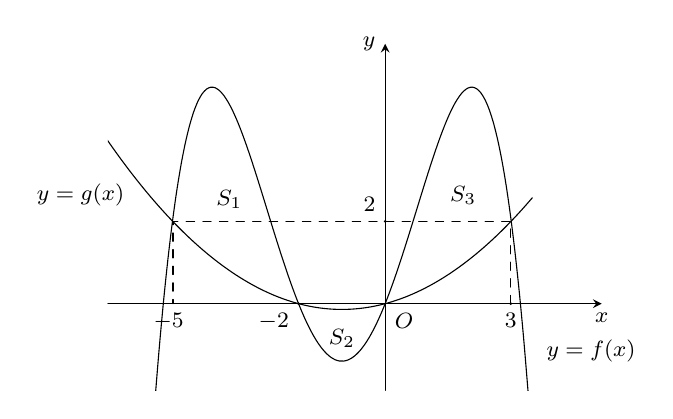
\begin{tikzpicture}[scale=.55,>=stealth, font=\footnotesize, line join=round, line cap=round]
\draw[->] (-6.4,0)--(5,0) node [below]{$x$};
\draw[->] (0,-2)--(0,6) node [left]{$y$};
\node at (0,0) [below right]{$O$};
\begin{scope}
\clip (-6.4,-2) rectangle (5,6);
\draw[smooth,samples=100,domain=-6.7:3.4] plot(\x,{0.133333*(\x)^2+0.266666*(\x)});
\draw[smooth,samples=100,domain=-6.5:3.3] plot(\x,{-0.078125*(\x)^4-0.3125*(\x)^3+0.9375*(\x)^2+2.5*(\x)});
\end{scope}
\draw[dashed](2.9,0)--(2.9,1.9)--(-4.9,1.9)--(-4.9,0) ;
\fill (-5,0) node[below]{$-5$}(-2,0) circle(1pt)node[below left]{$-2$}(0,1.9) circle(1pt)node[above left]{$2$}(2.9,0) circle(1pt)node[below]{$3$}  ;
\path (-3.6,2.4) node {$S_1$}
(-1,-0.8) node{$S_2$} (1.8,2.5) node{$S_3$}
(-5.8,2.5) node[left] {$y=g(x)$} (3.5,-1.1) node[right]{$y=f(x)$}
;
\end{tikzpicture}
}
\loigiai{
Đồ thị hàm số $g(x)=ax^2+bx+c$ đi qua các điểm $O\left(0;0\right)$, $A\left(-2;0\right)$, $B\left(3;2\right)$ nên   $g(x)=\dfrac{2}{15}x^2+\dfrac{4}{15}x$.\\
Từ hình vẽ, ta có
\begin{align*}
m-n+p&=\displaystyle\int\limits_{-5}^{-2}{\left[f(x)-g(x)\right]\mathrm{\,d}x}-\displaystyle\int\limits_{-2}^0{\left[g(x)-f(x)\right]\mathrm{\,d}x}+\displaystyle\int\limits_0^3{\left[f(x)-g(x)\right]\mathrm{\,d}x}\\
&=\displaystyle\int\limits_{-5}^3{f(x)\mathrm{\,d}x}-\displaystyle\int\limits_{-5}^3{g(x)\mathrm{\,d}x}
\end{align*}
Suy ra $$\displaystyle\int\limits_{-5}^3{f(x)\mathrm{\,d}x}=m-n+p+\displaystyle\int\limits_{-5}^3g(x)\mathrm{\,d}x=m-n+p+\displaystyle\int\limits_{-5}^3 \left (\dfrac{2}{15}x^2+\dfrac{4}{15}x\right )\mathrm{\,d}x=m-n+p+\dfrac{208}{45}.$$
}
\end{ex}


\begin{ex}%[Thi thử, THPT Gia Định HCM 2023]%[Phạm Tuấn, 12-EX6-2023]%[2D1K5-3]
Cho $g(x)=x^2-2x-1$ và hàm số $y=f(x)$ có bảng biến thiên như hình vẽ
\begin{center}

\begin{tikzpicture}
\tkzTabInit[lgt=1.2,espcl=2.5]
{$x$/0.8, $f’(x)$/0.8, $f(x)$/2.2}
{$-\infty$,$-2$,$1$,$+\infty$}
\tkzTabLine{ ,+,0,-,0,+, }
\tkzTabVar{-/$-\infty$,+/$1$,-/$-2$,+/$+\infty$}
\end{tikzpicture}
\end{center}
Số nghiệm của phương trình $f\left[g(x)\right]=0$ là
\choice
{$5$}
{\True $4$}
{$2$}
{$6$}
\loigiai{
Dựa vào bảng biến thiên ta có $f(x)=0\Leftrightarrow \hoac{& x=a\in (-\infty ;-2) \\&
x=b\in (-2;1) \\&
x=c\in (1;+\infty).}$\\
Suy ra $f\left[g(x)\right]=0\Leftrightarrow \hoac{& g(x)=a\in (-\infty ;-2) \\&g(x)=b\in (-2;1) \\&g(x)=c\in (1;+\infty).}$\\
Xét $g(x)=x^2-2x-1$, ta có $g'(x)=2x-2$;  $g'(x)=0\Leftrightarrow x=1$.\\
Bảng biến thiên
\begin{center}

\begin{tikzpicture}
\tkzTabInit[lgt=1.2,espcl=2.5]
{$x$/0.8, $g’(x)$/0.8, $g(x)$/2.2}
{$-\infty$,$1$,$+\infty$}
\tkzTabLine{ ,-,0,+, }
\tkzTabVar{+/$+\infty$,-/$-2$,+/$+\infty$}
\end{tikzpicture}
\end{center}
Từ bảng biến thiên suy ra:
\begin{itemize}
\item Phương trình $g(x)=a\in (-\infty ;-2)$ vô nghiệm.
\item Phương trình $g(x)=b$ có $2$ nghiệm phân biệt. 
\item Phương trình $g(x)=c$ có $2$ nghiệm phân biệt.
\end{itemize}
Vậy $f\left[g(x)\right]=0$ có $4$ nghiệm phân biệt.
}
\end{ex}


\begin{ex}%[Thi thử, THPT Gia Định HCM 2023]%[Phạm Tuấn, 12-EX6-2023]%[2H1K3-2]
Cho hình chóp $S.ABCD$ có đáy $ABCD$ là hình chữ nhật, $AD=2\sqrt{2}, AB=1$, $SA=SB, SC=SD$. Biết rằng hai mặt phẳng $(SAB)$ và $(SCD)$ vuông góc với nhau và tổng diện tích của hai tam giác $SAB$ và $SCD$ bằng $\sqrt{3}$. thể tích của khối chóp $S.ABCD$ bằng
\choice
{$1$}
{$\dfrac{4\sqrt{2}}{3}$}
{\True $\dfrac{2}{3}$}
{$\sqrt{2}$}
\loigiai{
\immini{
Gọi $d$ là giao tuyến của $(SAB)$ và $(SCD)$, dễ thấy $AB \parallel CD \parallel d$. \\
Gọi $M$, $N$ lần lượt là trung điểm của $AB$, $CD$. Tam giác $SAB$ cân tại $S$ suy ra $SM\perp AB$, mà $d \parallel AB$ do dó $SM\perp d$. \\
Mà $(SAB)\perp (SCD)$ suy ra $SM\perp (SCD)$,   suy ra $SM\perp SN$ hay tam giác $SMN$ vuông tại $S$.\\
Ta có $S_{\triangle SAB}+S_{\triangle SCD}=\sqrt{3}$ $\Leftrightarrow \dfrac{1}{2}\cdot AB\cdot SM+\dfrac{1}{2}\cdot CD\cdot SN=\sqrt{3}$\\ $\Rightarrow SM+SN=2\sqrt{3}$.\\
Tam giác $SMN$ vuông tại $S$ nên $SM^2+SN^2=MN^2={{(2\sqrt{2})}^2}=8$.\\
Ta có hệ phương trình $\heva{& SM+SN=2\sqrt{3} \\& SM^2+SN^2=8.}$
}
{
\begin{tikzpicture}[scale=0.77, font=\footnotesize, line join=round, line cap=round, >=stealth]
\path
(0,0) coordinate (A)
(4,0) coordinate (D)
(-140:0.6*4) coordinate (B)
($(B)+(D)-(A)$) coordinate (C)
($(A)!0.5!(B)$) coordinate (M)
($(C)!0.5!(D)$) coordinate (N)
(1.1,4) coordinate (S)
($(M)!(S)!(N)$) coordinate (H)
;
\draw (S)--(B)--(C)--(D)--(S)--(C) (S)--(N);
\draw[dashed] (H)--(S)--(A)--(B) (A)--(D) (S)--(M)--(N) ;
\draw    pic["", draw=black, angle eccentricity=0.75, angle radius=0.2cm]
{right angle=S--H--N};
\foreach \x/\g in {S/90,A/160,B/-120,C/-40,D/0, M/-90, N/-30, H/-90}
\fill[black] (\x) circle (1pt)+(\g:.3)node{$\x$};
\end{tikzpicture}
}
\noindent 
Suy ra $SM \cdot SN = \dfrac{(SM+SN)^2-SM^2-SN^2}{2} = 2$.  \\
Kẻ $SH\perp MN$,  suy ra  $SH\perp (ABCD)$.\\
Tam giác $SMN$ vuông tại $S$ nên $SH=\dfrac{SM\cdot SN}{MN}=\dfrac{1}{\sqrt{2}}$.\\
Vậy thể tích khối chóp $V_{SABCD}=\dfrac{1}{3}\cdot S_{ABCD}\cdot SH=\dfrac{2}{3}$.
}
\end{ex}


\begin{ex}%[Thi thử, THPT Gia Định HCM 2023]%[Phạm Tuấn, 12-EX6-2023]%[2D3K3-1]
Cho hàm số $f(x)=x^4+bx^2+c$ $\left(b,c\in \mathbb{R}\right)$ có đồ thị là đường cong $(C)$ và đường thẳng $(d)\colon y=g(x)$ tiếp xúc với $(C)$ tại điểm $x_0=1$. Biết $(d)$ và $(C)$ còn hai điểm chung khác có hoành độ là $x_1,x_2\left(x_1<x_2\right)$ và $\displaystyle\int\limits_{x_1}^{x_2}\dfrac{g(x)-f(x)}{(x-1)^2}\mathrm{\,d}x=\dfrac{4}{3}$. Tính diện tích hình phẳng giới hạn bởi đường cong $(C)$ và đường thẳng $(d)$.
\choice
{\True $\dfrac{29}{5}$}
{$\dfrac{28}{5}$}
{$\dfrac{143}{5}$}
{$\dfrac{43}{5}$}
\loigiai{
Theo giả thiết ta có $f(x)-g(x)=(x-1)^2\left(x-x_1\right)\left(x-x_2\right)=x^4+bx^2-mx+n. \quad (*)$\\
Ta có 
\begin{align*}
\int\limits_{x_1}^{x_2}\dfrac{f(x)-g(x)}{(x-1)^2}\mathrm{\,d}x &=\displaystyle\int\limits_{x_1}^{x_2}\left(x-x_1\right)\left(x-x_2\right)\mathrm{\,d}x =\displaystyle\int\limits_{x_1}^{x_2}{\left(x-x_1\right)\left(x-x_1+x_1-x_2\right)\mathrm{\,d}x} \\
& =\displaystyle\int\limits_{x_1}^{x_2}\left[\left(x-x_1\right)^2 + \left(x-x_1\right)\left(x_1-x_2\right)\right]\mathrm{\,d}x 
=\left[\dfrac{\left(x-x_1\right)^3}{3}+\left(x_1-x_2\right)\dfrac{\left(x-x_1\right)^2}{2}\right]\bigg|_{x_1}^{x_2} \\
& =\dfrac{\left(x_2-x_1\right)^3}{3}-\dfrac{\left(x_2-x_1\right)^3}{2}=-\dfrac{\left(x_2-x_1\right)^3}{6}=\dfrac{-4}{3}.
\end{align*}
Suy ra $\left(x_2-x_1\right)^3=8\Leftrightarrow x_2-x_1=2.\quad (1)$\\
Mặt khác theo định lí Vi-ét bậc 4 của phương trình $(*)$ suy ra
$1+1+x_2+x_1=0\Leftrightarrow x_2+x_1=-2. \quad (2)$\\
Từ $(1),(2)$ ta nhận được  $\heva{& x_2=0 \\& x_1=-2. }$\\
Vậy diện tích hình phẳng giới hạn bởi đường cong $(C)$ và đường thẳng $(d)$ là
$$S=\displaystyle\int\limits_{-2}^1\left| (x-1)^2(x+2)x \right|\mathrm{\,d}x=\dfrac{29}{5}.$$
}
\end{ex}


\begin{ex}%[Thi thử, THPT Gia Định HCM 2023]%[Phạm Tuấn, 12-EX6-2023]%[2H2K1-2]
Cho hình nón đỉnh $S$, đáy là hình tròn tâm $O$, góc ở đỉnh của hình nón là $\varphi =120^\circ$. Cắt hình nón bởi mặt phẳng đi qua đỉnh $S$ được thiết diện là tam giác vuông $SAB$, trong đó $A,B$ thuộc đường tròn đáy. Biết rằng khoảng cách giữa $SO$ và $AB$ bằng $3$. Diện tích xung quanh của hình nón bằng
\choice
{$\text{36}\sqrt{3}\pi$}
{\True $\text{18}\sqrt{3}\pi$}
{$\text{27}\sqrt{3}\pi$}
{$\text{9}\sqrt{3}\pi$}
\loigiai{
\immini
{
Kẻ $OH\perp AB$, ta lại có $OH\perp SO$ nên $\mathrm{d}(AB;SO)=OH=3$.\\
Tam giác $SAB$ vuông cân tại $S$ nên $AB=SB\sqrt{2}$. \\
Gọi $r$ là bán kính đường tròn đáy của hình nón.\\
Đường sinh $\ell =SB=\dfrac{OB}{\sin \widehat{OSB}}=\dfrac{r}{\sin 60^\circ }=\dfrac{2r\sqrt{3}}{3}$.\\
Suy ra $BH=\dfrac{AB}{2}=\dfrac{SB\sqrt{2}}{2}=\dfrac{r\sqrt{6}}{3}$.\\
Tam giác $OBH$ vuông tại $H$ nên
$$OH^2+BH^2=OB^2\Leftrightarrow 9+\dfrac{6r^2}{9}=r^2\Leftrightarrow r=3\sqrt{3}\Rightarrow \ell =\dfrac{2r\sqrt{3}}{3}=6.$$
Diện tích xung quanh $S_{\text{xq}}$ của hình nón là $S_{\text{xq}}=\pi r\ell =\pi \cdot 3\sqrt{3}\cdot 6=18\pi \sqrt{3}$.
}
{
\begin{tikzpicture}[scale=1, font=\footnotesize, line join=round, line cap=round, >=stealth]
\coordinate (C) at (0,0);
\coordinate (A) at (5,0);
\coordinate (O) at ($(C)!0.5!(A)$);
\coordinate (S) at ($(O)+(0,4)$);
\draw[dashed] (A) arc (0:180:2.5 cm and 0.6 cm);
\draw (A) arc (0:-180:2.5cm and 0.6 cm);
\coordinate (B) at ($(O)+({2.5*cos(-110)},{0.6*sin(-110)})$);
\coordinate (H) at ($(A)!0.5!(B)$);
\tkzDrawSegments(S,C S,A S,B)
\tkzDrawSegments[dashed](H,A S,O B,A O,B S,H O,A O,H)
\draw    
pic["", draw=black, angle eccentricity=0.75, angle radius=0.2cm]{right angle=O--H--B}
pic["", draw=black, angle eccentricity=0.75, angle radius=0.2cm] {right angle=S--O--A};
\foreach \x/\g in {A/0,B/-90,S/90,H/-30,O/160} 
\fill[black](\x) circle (1pt)+(\g:3mm) node{$\x$};
\end{tikzpicture}
}
}
\end{ex}


\begin{ex}%[Thi thử, THPT Gia Định HCM 2023]%[Phạm Tuấn, 12-EX6-2023]%[2D4G5-1]
Cho hai số phức $z_1,z_2$ thỏa mãn $\left| z_1+2-i \right|+\left| z_1-4-7i \right|=6\sqrt{2}$ và $\left| iz_2-1+2i \right|=1$. Giá trị nhỏ nhất của biểu thức $P=\left| z_1+z_2 \right|$ bằng
\choice
{$\text{3}\sqrt{2}-2$}
{$\text{2}\sqrt{2}-2$}
{$\text{3}\sqrt{2}-1$}
{\True $\text{2}\sqrt{2}-1$}
\loigiai{
Gọi $A$, $B$, $M$ lần lượt là điểm biểu diễn số phức $-2+i$; $4+7i$; $z_1$, khi đó 
$$\left| z_1+2-i \right|+\left| z_1-4-7i \right|=6\sqrt{2}\Leftrightarrow MA+MB=6\sqrt{2}.$$
Mà  $AB=6\sqrt{2}$, suy ra  $MA+MB=AB$ hay $M$ thuộc đoạn thẳng $AB$.\\
Ta có $\left| iz_2-1+2i \right|=1 \Leftrightarrow |-z_2-2-i| = 1$. 
\begin{center}
\begin{tikzpicture}[scale=0.55, font=\footnotesize, line join=round, line cap=round, >=stealth]
\path
(-2,1) coordinate (A)
(3,5) coordinate (B)
(2,1) coordinate (I)
($(A)!0.7!(B)$) coordinate (M)
(0,0) coordinate (O)
($(I)+(80:1cm)$) coordinate (N)
;
\draw[->] (-3,0)--(5,0) node[below]{$x$};
\draw[->] (0,-1)--(0,6) node[left]{$y$};
\draw[thick] (M)--(N) (A)--(B) ;
\draw[thick] (I) circle(1) ;
\foreach \x/\g in{A/-120,B/50,M/100,N/60,I/-30,O/-140}
\fill[black](\x)circle(1.1pt) ($(\x)+(\g:5mm)$) node{$\x$}; 
\end{tikzpicture}
\end{center}
Gọi $N$, $I$ là điểm biểu diễn số phức $-z_2$ và $2+i$, khi đó $|-z_2-2-i| = 1\Leftrightarrow NI=1$.\\
Suy ra  $N$ nằm trên đường tròn tâm $I(2;1)$, bán kính $R=1$.\\
Ta có $P=\left| z_1+z_2 \right|=\left| z_1-\left(-z_2\right) \right|=MN$.\\
PTĐT $AB\colon x-y+3=0$; $\mathrm{d}(I;AB)=2\sqrt{2}$.\\
Khi đó,  $P_{\min}=\mathrm{d}(I;AB)-R=2\sqrt{2}-1$.
}
\end{ex}


\begin{ex}%[Thi thử, THPT Gia Định HCM 2023]%[Phạm Tuấn, 12-EX6-2023]%[2H3G3-8]
Trong KG $Oxyz$, cho mặt phẳng $(P)\colon x-y+z+7=0$, đường thẳng $d\colon \dfrac{x}{1}=\dfrac{y}{-2}=\dfrac{z}{2}$ và mặt cầu $(S)\colon (x-1)^2+y^2+(z-2)^2=5$. Gọi $A$, $B$ là hai điểm trên mặt cầu $(S)$ và $AB=4$;  $A'$, $B'$ là hai điểm nằm trên mặt phẳng $(P)$ sao cho $AA',BB'$ cùng song song với đường thẳng $d$. Giá trị lớn nhất của tổng $AA'+BB'$ gần nhất với giá trị nào sau đây?
\choice
{$13$}
{$11$}
{$12$}
{\True $14$}
\loigiai{
\begin{center}
\begin{tikzpicture}[scale=1, font=\footnotesize, line join=round, line cap=round, >=stealth]
\path
(3,4) coordinate (I)
(1.4,4.5) coordinate (A)
(3.6,3.2) coordinate (B)
(0.77,1) coordinate (A')
(3.1,0.2) coordinate (B')
($(A)!0.3!(A')$) coordinate (A1)
($(A)!0.5!(B)$) coordinate (M)
($(A')!0.5!(B')$) coordinate (M')
($(M)!0.2!(M')$) coordinate (M1)
(2.6,1.1) coordinate (H)
(0,2) coordinate (X)
(-1.5,-0.5) coordinate (Y)
(4.5,-0.5) coordinate (Z)
($(X)+(Z)-(Y)$) coordinate (T)
;
\draw[fill=cyan!30,thick] (I) circle (2);
\draw  (A1)--(A')--(B')--(B) (M')--(M1)  ;
\draw [dashed] (A1)--(A)--(B) (M1)--(M)--(H)--(M') ;
\coordinate  (K) at (5,4) ;
\draw [dashed] (K) arc (0:180:2cm and 0.4cm);
\draw  (K) arc (0:-180:2cm and 0.4cm);
\draw[thick] (X)--(Y)--(Z)--(T);
\draw pic["$P$", draw=black, angle eccentricity=0.55, angle radius=1cm]{angle=Z--Y--X};
\foreach \x/\g in{A/80,B/20,A'/-120,B'/-90,M/90,M'/-90,I/30,H/-30}
\fill[black](\x)circle(1.1pt) ($(\x)+(\g:2.5mm)$) node{$\x$}; 
\end{tikzpicture}
\end{center}
Mặt cầu $(S)$ có tâm $I(1;0;2)$ và bán kính $R=\sqrt{5}$.\\
$\mathrm{d}  \left(I;(P)\right)=\dfrac{10\sqrt{3}}{3}>R$ nên $(P)$ và mặt cầu $(S)$ không giao nhau.\\
Gọi $M$ là trung điểm của $AB$, $M'$ là trung điểm của $A’ B’$. Dễ thấy $MM'$ song song hoặc trùng $d$ và $AA'+BB'=2MM'$. \\
Gọi $H$ là hình chiếu vuông góc của $M$ trên $(P)$. Ta có 
$$AA’ +BB’ =2MM'=\dfrac{2MH}{\sin \widehat{HM'M}}=\dfrac{2MH}{\sin \left(d;(P)\right)}. $$
Ta có $\sin \left(d;(P)\right)=\sin \left(d;(P)\right)=\dfrac{5\sqrt{3}}{9}$. Do đó $AA’ +BB’$ lớn nhất khi $MH$ lớn nhất. \\
Theo giả thiết $AB=4$, suy ra $IM=\sqrt{R^2-AM^2} = 1$. Do đó $M$ thuộc mặt cầu $(\mathcal{C})$, tâm $I$, bán kính $r = 1$. \\
Khi đó,  $MH_{\max }=r+\mathrm{d}\left(I;(P)\right)=1+\dfrac{10\sqrt{3}}{3}=\dfrac{3+10\sqrt{3}}{3}$.\\
Vậy giá trị lớn nhất của $AA'+\,BB'$ bằng $2\cdot \dfrac{\dfrac{3+10\sqrt{3}}{3}}{\dfrac{5\sqrt{3}}{9}}\approx 14$.
}
\end{ex}


\begin{ex}%[Thi thử, THPT Gia Định HCM 2023]%[Phạm Tuấn, 12-EX6-2023]%[2D2G6-2]
Có bao nhiêu giá trị nguyên của tham số $m$ để tập nghiệm của bất phương trình
$$2023^{\ln \left(2x^2+4x+m\right)}-2023^{2\ln (2x-1)}>0$$ chứa đúng bốn số nguyên?
\choice
{$16$}
{\True $10$}
{$11$}
{$9$}
\loigiai{
Điều kiện $\heva{& 2x-1>0 \\& 2x^2+4x+m>0 }\Leftrightarrow \heva{& x>\dfrac{1}{2} \\& 2x^2+4x+m>0.}$\\
Ta có 
\begin{align*}
&2023^{\ln \left(2x^2+4x+m\right)}-2023^{2\ln (2x-1)}>0 \\
\Leftrightarrow~& \ln \left(2x^2+4x+m\right)>2\ln (2x-1)\\
\Leftrightarrow~& 2x^2+4x+m>(2x-1)^2 \\
\Leftrightarrow~& m>2x^2-8x+1.
\end{align*}
Xét $f(x)=2x^2-8x+1$ với $x>\dfrac{1}{2}$.\\
Ta có bảng biến thiên
\begin{center}

\begin{tikzpicture}
\tkzTabInit[lgt=1.2,espcl=1.8]
{$x$/1, $g(x)$/2.2}
{$\dfrac{1}{2}$,$1$, $2$,$3$, $4$, $5$}
\tkzTabVar{+/$-2{,}5$, R,  -/$-7$, R, R, +/$11$}
\tkzTabVal{3}{6}{2/3}{$4$}{$1$}
\end{tikzpicture}
\end{center}
Tập nghiệm của bất phương trình chứa đúng $4$ số nguyên khi và chỉ khi  $1<m\le 11$.\\
Vậy có $10$ giá trị nguyên $m$ thỏa mãn.
}
\end{ex}


\begin{ex}%[Thi thử, THPT Gia Định HCM 2023]%[Phạm Tuấn, 12-EX6-2023]%[2D2G4-3]
Cho hàm số $f(x)=\ln ^3x+6(m-1)\ln ^2x-3m^2\ln x+4$. Biết rằng đoạn [a, b] là tập hợp tất cả các giá trị của tham số $m$ để hàm số $y=|f(x)|$ đồng biến trên khoảng $(\mathrm{e}  ;+\infty)$. Giá trị biểu thức $a+3b$ bằng
\choice
{\True $4+\sqrt{6}$}
{$12+2\sqrt{6}$}
{}
{3}
\loigiai{
Ta có $f'(x) = \dfrac{3\ln ^2x+12(m-1)\ln x-3m^2}{x}$. \\
Đặt $t=\ln x$, $x\in (\mathrm{e};+\infty) \Rightarrow  t\in (1;+\infty)$.\\
Xét hàm số $g(t)=t^3+6(m-1)t^2-3m^2t+4$ trên khoảng $(1;+\infty)$.\\
Ta có $g'(t)=3t^2+12(m-1)t-3m^2$ và $ \lim\limits_{t\to +\infty } g'(t)=+\infty $. \\
Hàm số $y=|f(x)|$ đồng biến trên khoảng $(1;+\infty)$ 
\[ 
\Leftrightarrow \heva{& f'(x)\ge 0,\forall x\in (\mathrm{e};+\infty) \\& f(\mathrm{e})\ge 0 }
\Leftrightarrow \heva{& g'(t)\ge 0,\forall t\in (1;+\infty) && (1) \\& g(1)\ge 0. && (2)}
\]
$\bullet$ $(2)\Leftrightarrow  -3m^2+6m-1\ge 0\Rightarrow \dfrac{3-\sqrt{6}}{3}\le m\le \dfrac{3+\sqrt{6}}{3}$.  \quad (3)\\
$\bullet$ Từ (1), ta có $\Delta' = 36(m-1)^2+9m^2>0,\forall m$, suy ra  $g'(t)$ luôn có 2 nghiệm $t_1$, $t_2$.  \\
Bảng xét dấu của $g'(t)$
\begin{center}

\begin{tikzpicture}
\tkzTabInit[lgt=1.2,espcl=2.5]
{$t$/0.7, $g’(t)$/0.7}
{$-\infty$, $t_1$, $t_2$, $+\infty$}
\tkzTabLine{ ,+,0,-,0,+, }
\end{tikzpicture}
\end{center}
Do đó
\begin{align*}
(1) &\Leftrightarrow  t_2=-2(m-1)+\sqrt{5m^2-8m+4}\le 1 \\
&\Leftrightarrow \sqrt{5m^2-8m+4}\le 2m -1 \\
&\Leftrightarrow \heva{&2m-1 \geq 0\\&5m^2-8m+4 \geq 0\\& 5m^2-8m+4 \le (2m-1)^2} \\
&\Leftrightarrow 1\le m\le 3.  \quad (4)
\end{align*}
Kết hợp $(3)$ và $(4)$ ta được $m\in \left[1;\dfrac{3+\sqrt{6}}{3}\right]\Rightarrow a=1$; $b=\dfrac{3+\sqrt{6}}{3}$.\\
Vậy $a+3b=4+\sqrt{6}$.
}
\end{ex}
\Closesolutionfile{ans}
\begin{indapan}{10}
	{ans/ans-2-TT-13-GiaDinh-HCM-23}
\end{indapan}
